% This is samplepaper.tex, a sample chapter demonstrating the
% LLNCS macro package for Springer Computer Science proceedings;
% Version 2.21 of 2022/01/12
%
\documentclass[runningheads]{llncs}
%
\usepackage[T1]{fontenc}
% T1 fonts will be used to generate the final print and online PDFs,
% so please use T1 fonts in your manuscript whenever possible.
% Other font encondings may result in incorrect characters.
%
\usepackage{graphicx}
% Used for displaying a sample figure. If possible, figure files should
% be included in EPS format.
%
% If you use the hyperref package, please uncomment the following two lines
% to display URLs in blue roman font according to Springer's eBook style:
%\usepackage{color}
%\renewcommand\UrlFont{\color{blue}\rmfamily}
%\urlstyle{rm}

\usepackage{amsmath}
\usepackage{marvosym}
\usepackage{hyperref}

\def\letter{$^{\textrm{(\Letter)}}$}

\begin{document}
%
\title{Parallel algorithm for solving multicriterial optimization problems using elements of machine learning}
%
\titlerunning{Parallel algorithm for solving multicriterial optimization problems}
% If the paper title is too long for the running head, you can set
% an abbreviated paper title here
%
\author{{Sergey Konnov\orcidID{0009-0003-4590-0870} \and
Evgeny Kozinov \Letter\orcidID{0000-0001-6776-0096} \and
Konstantin Barkalov \orcidID{0000-0001-5273-2471} \and
Alexander Sysoyev \orcidID{0000-0003-1542-7624} \and
Vladimir Grishagin\orcidID{0000-0002-2884-3670}}
}
%
\authorrunning{S. Konnov, E. Kozinov, K. Barkalov, A. Sysoyev and V. Grishagin}
% First names are abbreviated in the running head.
% If there are more than two authors, 'et al.' is used.
%
\institute{Lobachevsky State University of Nizhni Novgorod, Nizhni Novgorod, Russia 
\email{\{konstantin.barkalov,evgeny.kozinov\}@itmm.unn.ru}, \email{vagris@unn.ru}}
%
\maketitle              % typeset the header of the contribution
%
\begin{abstract}
Solving problems of multi-criteria optimization involves finding many combinations of optimization parameters, in which the values of the criteria cannot be improved in several criteria at once without worsening the values   of the remaining ones (Pareto set). In the framework of the research, several assumptions were introduced: criteria are multiextremal and difficult to calculate, presented in the form of a ``black box'', and the number of optimized parameters is small. The paper presents a method for solving this class of problems based on the information-statistical approach and a machine learning procedure used to increase search efficiency. A parallel implementation of the method is described, which is supplemented with the ability to perform calculations in asynchronous parallel mode. The efficiency and scalability of the proposed algorithm is analyzed on the base of solving a test class of multiextremal problems.



\keywords{Multicriterial Problems \and Global Optimization \and Machine Learning \and High Performance Computing.}
\end{abstract}
%
%
%

\section{Introduction}

\cite{Miettinen1999,Ehrgott2005,Pardalos2017,Konnov2025,Evtushenko2014,DPA02,Durillo2010,Mostaghim2007,Nebro2009,RC05,Zitzler2001,Gergel2019_2,Gergel2018,GergelKozinov2020,Marler2004,Strongin2000,Sergeyev2013,MCO_ML_2023,scikit-learn,PyTorch,ioptmco,HV,pymoo,AGP_ML}


\begin{figure}
\center
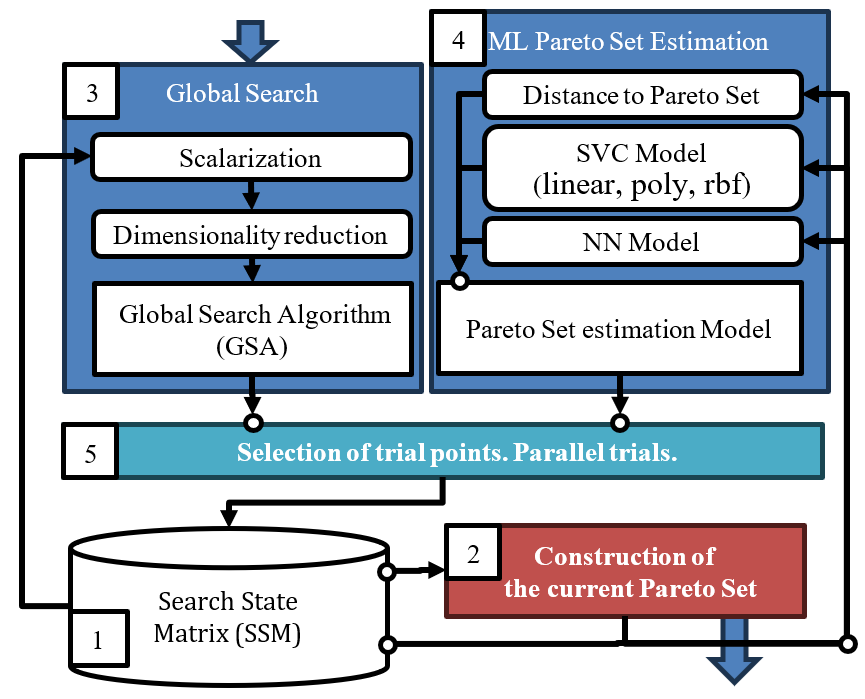
\includegraphics[width=0.6\textwidth]{fig1.png}
\caption{Computational scheme of the algorithm for solving multicriterial optimization problems using machine learning models.} \label{fig1}
\end{figure}

\begin{figure}
\center
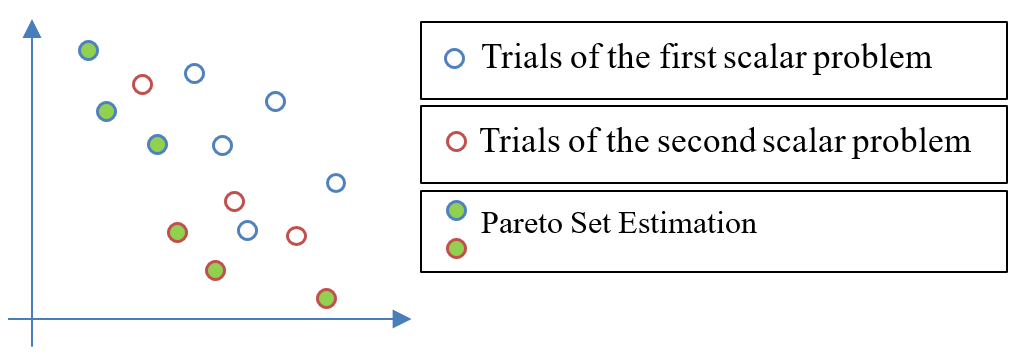
\includegraphics[width=0.6\textwidth]{fig2.png}
\caption{Example of Pareto set evaluation in solving two scalar optimization problems.} \label{fig2}
\end{figure}

\begin{figure}
\center
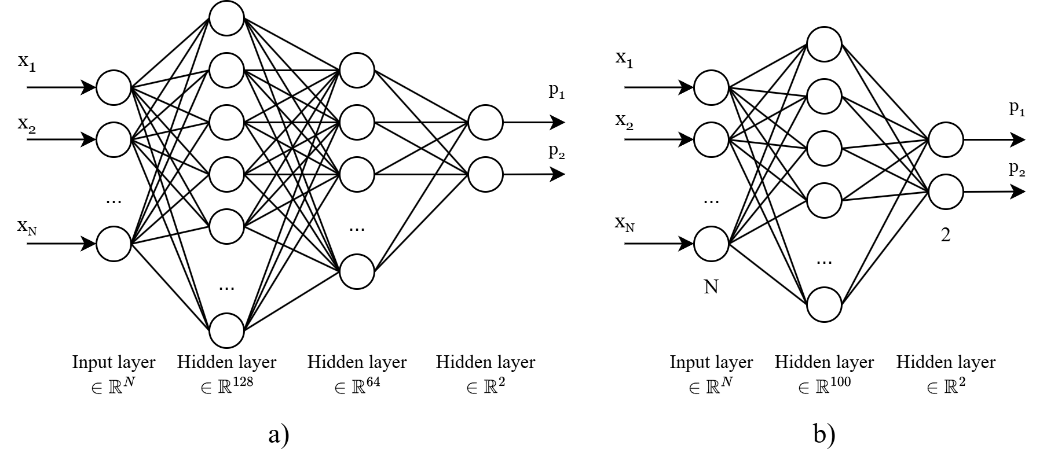
\includegraphics[width=0.8\textwidth]{fig3.png}
\caption{Neural network models used to calculate the characteristic $R_{PS}(i)$.} \label{fig3}
\end{figure}

\begin{figure}
\center
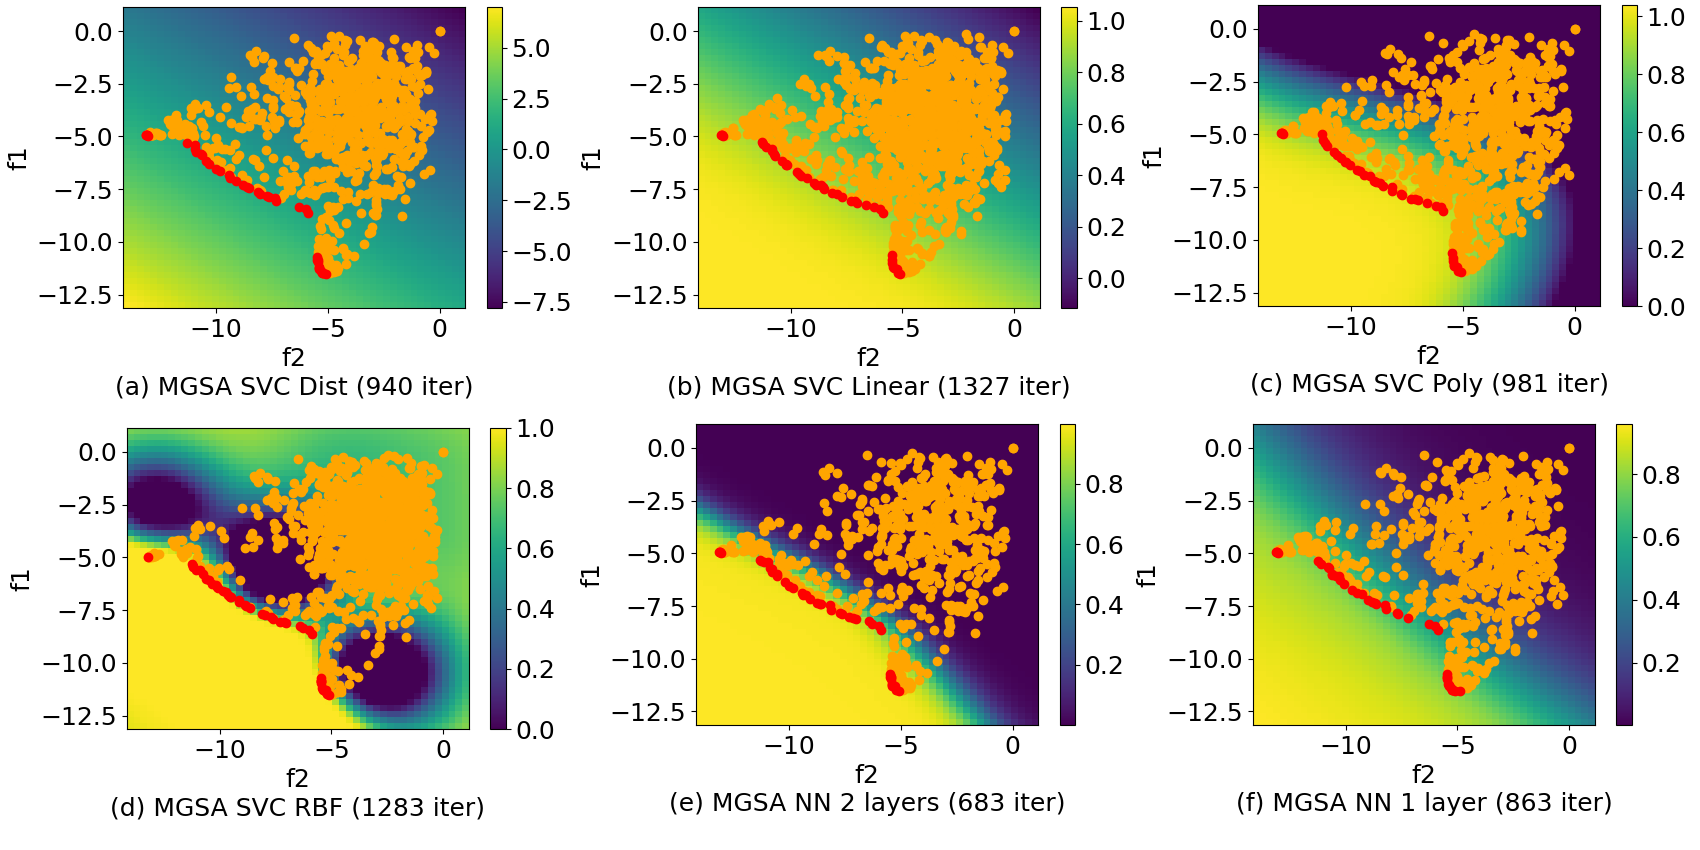
\includegraphics[width=0.6\textwidth]{fig4.png}
\caption{Examples of Pareto set evaluation for the case of two scalar optimization problems.} \label{fig4}
\end{figure}

\begin{figure}
\center
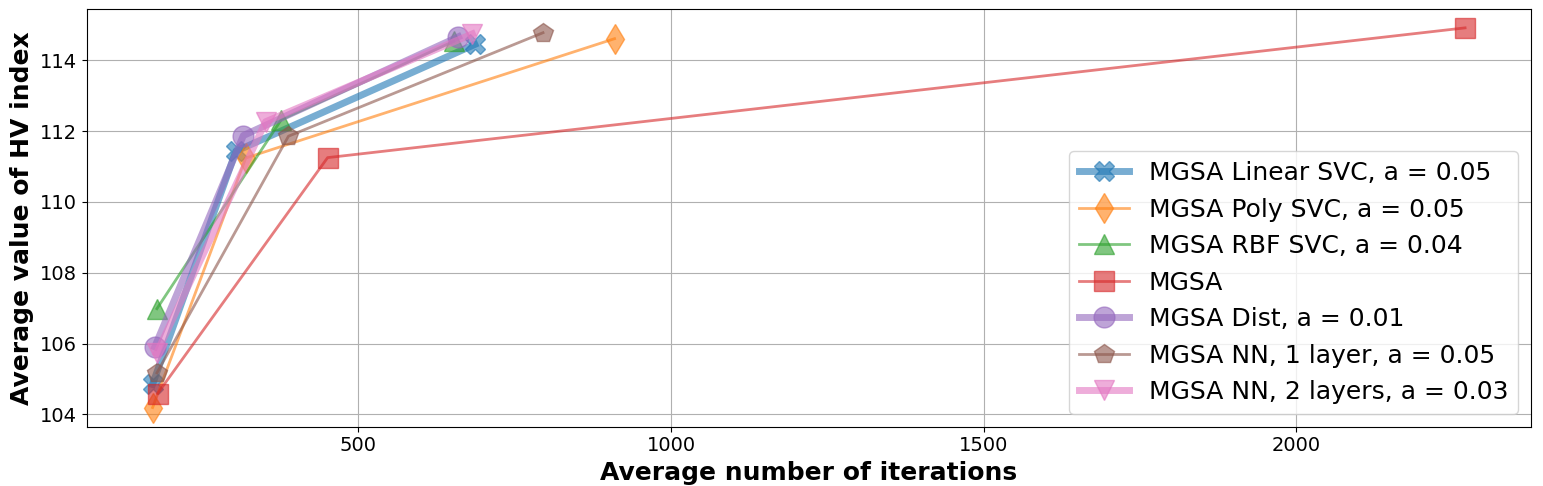
\includegraphics[width=0.8\textwidth]{fig5.png}
\caption{Comparison of HW index values for sequential algorithm implementation.} \label{fig5}
\end{figure}

\begin{figure}
\center
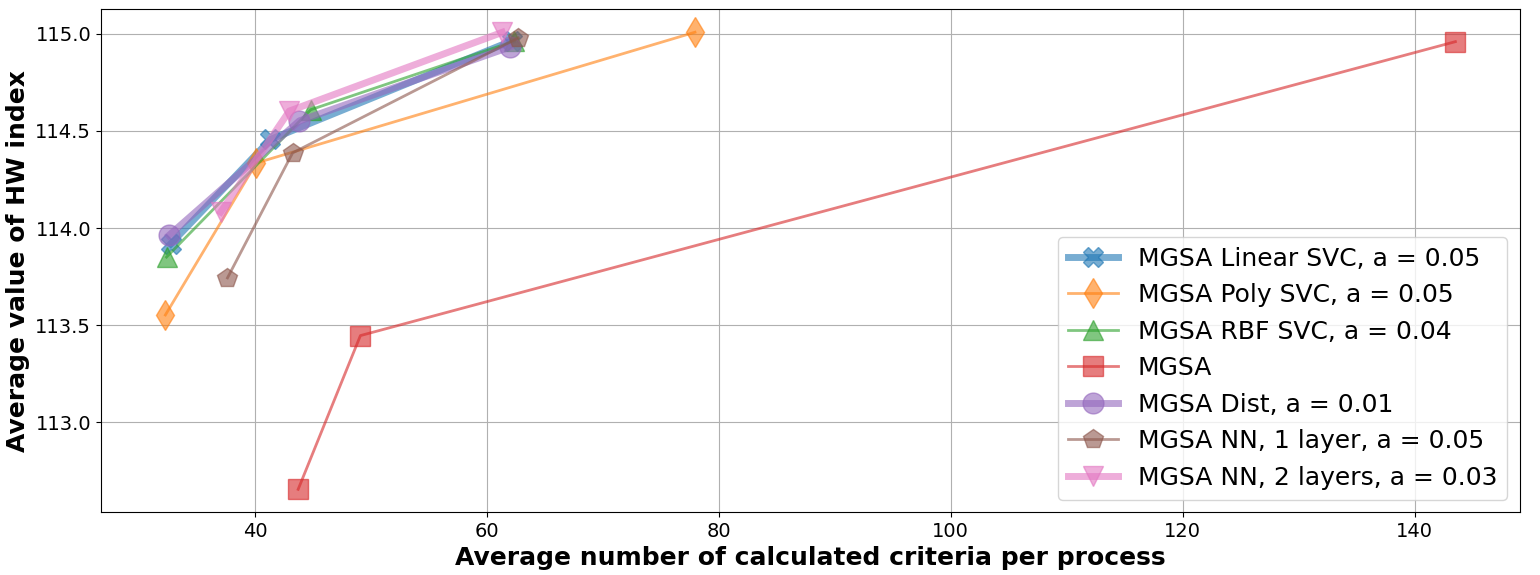
\includegraphics[width=0.8\textwidth]{fig6.png}
\caption{Dependence of the mean value of the index HW from the trial number per process for the case of 20 processes.} \label{fig6}
\end{figure}

\begin{figure}
\center
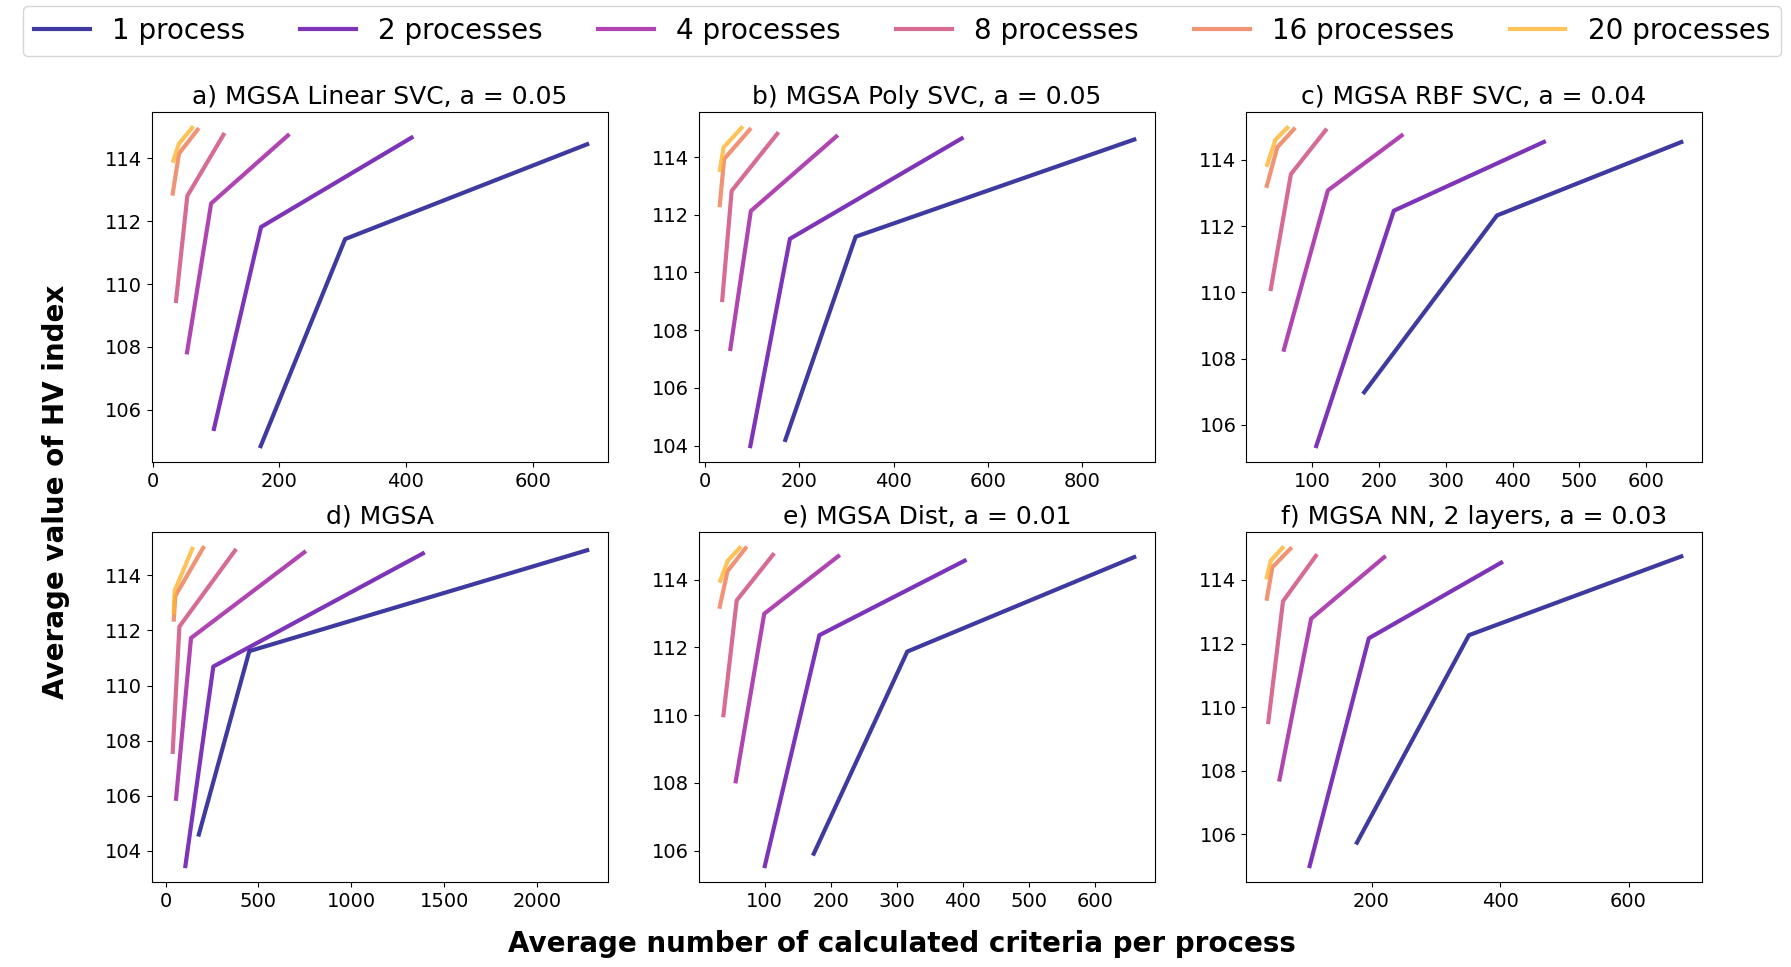
\includegraphics[width=0.8\textwidth]{fig7.png}
\caption{Dependence of the HW index on the number of trials executed for different number of processes.} \label{fig7}
\end{figure}



\begin{credits}
\subsubsection{\ackname} This study was funded by the ...

\subsubsection{\discintname}
The authors have no competing interests to declare that are relevant to the content of this article.
\end{credits}
%
% ---- Bibliography ----
%
% BibTeX users should specify bibliography style 'splncs04'.
% References will then be sorted and formatted in the correct style.
%
\bibliographystyle{splncs04}
\bibliography{bibliography}
%
%\begin{thebibliography}{8}
%\bibitem{ref_article1}
%Author, F.: Article title. Journal \textbf{2}(5), 99--110 (2016)
%
%\bibitem{ref_lncs1}
%Author, F., Author, S.: Title of a proceedings paper. In: Editor,
%F., Editor, S. (eds.) CONFERENCE 2016, LNCS, vol. 9999, pp. 1--13.
%Springer, Heidelberg (2016). \doi{10.10007/1234567890}
%
%\bibitem{ref_book1}
%Author, F., Author, S., Author, T.: Book title. 2nd edn. Publisher,
%Location (1999)
%
%\bibitem{ref_proc1}
%Author, A.-B.: Contribution title. In: 9th International Proceedings
%on Proceedings, pp. 1--2. Publisher, Location (2010)
%
%\bibitem{ref_url1}
%LNCS Homepage, \url{http://www.springer.com/lncs}, last accessed 2023/10/25
%\end{thebibliography}
\end{document}
